% Options for packages loaded elsewhere
\PassOptionsToPackage{unicode}{hyperref}
\PassOptionsToPackage{hyphens}{url}
%
\documentclass[
]{article}
\usepackage{amsmath,amssymb}
\usepackage{iftex}
\ifPDFTeX
  \usepackage[T1]{fontenc}
  \usepackage[utf8]{inputenc}
  \usepackage{textcomp} % provide euro and other symbols
\else % if luatex or xetex
  \usepackage{unicode-math} % this also loads fontspec
  \defaultfontfeatures{Scale=MatchLowercase}
  \defaultfontfeatures[\rmfamily]{Ligatures=TeX,Scale=1}
\fi
\usepackage{lmodern}
\ifPDFTeX\else
  % xetex/luatex font selection
    \setmainfont[Numbers=Lowercase,Numbers=Proportional]{Skolar PE}
    \setsansfont[]{Skolar Sans PE}
\fi
% Use upquote if available, for straight quotes in verbatim environments
\IfFileExists{upquote.sty}{\usepackage{upquote}}{}
\IfFileExists{microtype.sty}{% use microtype if available
  \usepackage[]{microtype}
  \UseMicrotypeSet[protrusion]{basicmath} % disable protrusion for tt fonts
}{}
\makeatletter
\@ifundefined{KOMAClassName}{% if non-KOMA class
  \IfFileExists{parskip.sty}{%
    \usepackage{parskip}
  }{% else
    \setlength{\parindent}{0pt}
    \setlength{\parskip}{6pt plus 2pt minus 1pt}}
}{% if KOMA class
  \KOMAoptions{parskip=half}}
\makeatother
\usepackage{xcolor}
\usepackage[top=20mm,left=25mm,right=25mm,bottom=20mm]{geometry}
\usepackage{longtable,booktabs,array}
\usepackage{calc} % for calculating minipage widths
% Correct order of tables after \paragraph or \subparagraph
\usepackage{etoolbox}
\makeatletter
\patchcmd\longtable{\par}{\if@noskipsec\mbox{}\fi\par}{}{}
\makeatother
% Allow footnotes in longtable head/foot
\IfFileExists{footnotehyper.sty}{\usepackage{footnotehyper}}{\usepackage{footnote}}
\makesavenoteenv{longtable}
\usepackage{graphicx}
\makeatletter
\newsavebox\pandoc@box
\newcommand*\pandocbounded[1]{% scales image to fit in text height/width
  \sbox\pandoc@box{#1}%
  \Gscale@div\@tempa{\textheight}{\dimexpr\ht\pandoc@box+\dp\pandoc@box\relax}%
  \Gscale@div\@tempb{\linewidth}{\wd\pandoc@box}%
  \ifdim\@tempb\p@<\@tempa\p@\let\@tempa\@tempb\fi% select the smaller of both
  \ifdim\@tempa\p@<\p@\scalebox{\@tempa}{\usebox\pandoc@box}%
  \else\usebox{\pandoc@box}%
  \fi%
}
% Set default figure placement to htbp
\makeatletter
\def\fps@figure{htbp}
\makeatother
\setlength{\emergencystretch}{3em} % prevent overfull lines
\providecommand{\tightlist}{%
  \setlength{\itemsep}{0pt}\setlength{\parskip}{0pt}}
\setcounter{secnumdepth}{-\maxdimen} % remove section numbering
% definitions for citeproc citations
\NewDocumentCommand\citeproctext{}{}
\NewDocumentCommand\citeproc{mm}{%
  \begingroup\def\citeproctext{#2}\cite{#1}\endgroup}
\makeatletter
 % allow citations to break across lines
 \let\@cite@ofmt\@firstofone
 % avoid brackets around text for \cite:
 \def\@biblabel#1{}
 \def\@cite#1#2{{#1\if@tempswa , #2\fi}}
\makeatother
\newlength{\cslhangindent}
\setlength{\cslhangindent}{1.5em}
\newlength{\csllabelwidth}
\setlength{\csllabelwidth}{3em}
\newenvironment{CSLReferences}[2] % #1 hanging-indent, #2 entry-spacing
 {\begin{list}{}{%
  \setlength{\itemindent}{0pt}
  \setlength{\leftmargin}{0pt}
  \setlength{\parsep}{0pt}
  % turn on hanging indent if param 1 is 1
  \ifodd #1
   \setlength{\leftmargin}{\cslhangindent}
   \setlength{\itemindent}{-1\cslhangindent}
  \fi
  % set entry spacing
  \setlength{\itemsep}{#2\baselineskip}}}
 {\end{list}}
\usepackage{calc}
\newcommand{\CSLBlock}[1]{\hfill\break\parbox[t]{\linewidth}{\strut\ignorespaces#1\strut}}
\newcommand{\CSLLeftMargin}[1]{\parbox[t]{\csllabelwidth}{\strut#1\strut}}
\newcommand{\CSLRightInline}[1]{\parbox[t]{\linewidth - \csllabelwidth}{\strut#1\strut}}
\newcommand{\CSLIndent}[1]{\hspace{\cslhangindent}#1}
\usepackage{indentfirst}
\setlength\parindent{24pt}
\usepackage[left]{lineno}
\modulolinenumbers[1]
\usepackage{multicol}
\usepackage{setspace}
\usepackage{float}
\usepackage{afterpage}
\usepackage{stfloats}
\usepackage{graphicx}
\newcommand{\hideFromPandoc}[1]{#1}
 \let\Begin\begin \let\End\end
\usepackage[labelfont=bf]{caption}
\captionsetup{labelfont=bf}
\usepackage{amsmath}
\DeclareMathOperator\arctanh{arctanh}
\makeatletter
\@ifpackageloaded{subfig}{}{\usepackage{subfig}}
\@ifpackageloaded{caption}{}{\usepackage{caption}}
\captionsetup[subfloat]{margin=0.5em}
\AtBeginDocument{%
\renewcommand*\figurename{Fig}
\renewcommand*\tablename{Table}
}
\AtBeginDocument{%
\renewcommand*\listfigurename{List of Figures}
\renewcommand*\listtablename{List of Tables}
}
\newcounter{pandoccrossref@subfigures@footnote@counter}
\newenvironment{pandoccrossrefsubfigures}{%
\setcounter{pandoccrossref@subfigures@footnote@counter}{0}
\begin{figure}\centering%
\gdef\global@pandoccrossref@subfigures@footnotes{}%
\DeclareRobustCommand{\footnote}[1]{\footnotemark%
\stepcounter{pandoccrossref@subfigures@footnote@counter}%
\ifx\global@pandoccrossref@subfigures@footnotes\empty%
\gdef\global@pandoccrossref@subfigures@footnotes{{##1}}%
\else%
\g@addto@macro\global@pandoccrossref@subfigures@footnotes{, {##1}}%
\fi}}%
{\end{figure}%
\addtocounter{footnote}{-\value{pandoccrossref@subfigures@footnote@counter}}
\@for\f:=\global@pandoccrossref@subfigures@footnotes\do{\stepcounter{footnote}\footnotetext{\f}}%
\gdef\global@pandoccrossref@subfigures@footnotes{}}
\@ifpackageloaded{float}{}{\usepackage{float}}
\floatstyle{ruled}
\@ifundefined{c@chapter}{\newfloat{codelisting}{h}{lop}}{\newfloat{codelisting}{h}{lop}[chapter]}
\floatname{codelisting}{Listing}
\newcommand*\listoflistings{\listof{codelisting}{List of Listings}}
\makeatother
\ifLuaTeX
  \usepackage{selnolig}  % disable illegal ligatures
\fi
\usepackage{bookmark}
\IfFileExists{xurl.sty}{\usepackage{xurl}}{} % add URL line breaks if available
\urlstyle{same}
\hypersetup{
  pdftitle={Super serious manuscript on imporant science},
  pdfauthor={Diogo Melo1,},
  pdfkeywords={modularity, gene
co-expression, WGCNA, MMC, clustering, RNA-seq, GO enrichment},
  hidelinks,
  pdfcreator={LaTeX via pandoc}}

\title{Super serious manuscript on imporant science}
\author{Diogo Melo\textsuperscript{1,*}}
\date{}

\newfontfamily\titlefont{Skolar Sans PE}

\usepackage{titlesec}
\newfontfamily\sectionfont{Skolar Sans PE}
\titleformat*{\section}{\Large\bfseries\sectionfont}
\titleformat*{\subsection}{\large\bfseries\sectionfont}
\titleformat*{\subsubsection}{\normalsize\bfseries\sectionfont}

\begin{document}
\makeatletter
\renewcommand{\maketitle}{\setlength{\parindent}{0pt}
\begin{flushleft}
    \huge{\titlefont \textbf{Super serious manuscript on imporant
science}}
    
          \vspace{0.2cm}
      \small{Manuscript v0.1 - \today}
    
    \vspace{0.2cm}

    \Large{Diogo Melo\textsuperscript{1,*}}

    \vspace{0.3cm}

\end{flushleft}
}
\makeatother
\maketitle



\footnotesize
\textsuperscript{1} Departamento de Genética e Biologia Evolutiva,
Instituto de Biociências, Universidade de São Paulo, São Paulo, SP,
Brasil

\href{mailto:damelo@ib.usp.br}{*damelo@ib.usp.br (DM)}

\normalsize

\section{Abstract}\label{abstract}

Evolutio genetica lorem ipsum dolor sit amet, consectetur adipiscing
elit. Mutatio DNA in populationes per tempus, selectio naturalis
adaptationesque. Hereditatem traits per generationes, geni fluxus in
ecosystemata. Variatio alleles frequentia, fitness reproductiva in
ambientia. Genomica comparativa revelavit homologiam inter species,
demonstrans communem originem. Epigenetica regulatio gene expressione
sine mutatione sequentiae DNA. Speciatio et divergentia per isolationem
reproductivam, accumulatio differentiarum geneticarum. Molecularis
horologia evolutionis, fossilia DNA ex speciminibus antiquis.
Horizontalis gene translatio inter bacterias, archaeas, et eucaryotas.
Coevolutio inter species symbioticas, Red Queen hypothesis in arms race
genetica. Pleiotropy, epistasis, et gene-environment interactiones in
phenotypica expressione. Neutral theory molecularis evolutionis, genetic
drift in populationes parvas. Balancing selectio et frequentia-dependens
selectio in polymorphismi conservatione. Evolutio convergenta in traits
similibus inter lineas non-related. Evolutio reticula in plantis et
bacteriis per hybridisationem et horizontalem gene translationem.
Evo-devo explorat genes regulatorias in evolutione morphologica.
Metagenomics revelat diversitatem microbialem incognitam in
ecosystematis. Evolutio resistentiae ad medicamenta in pathogenis et
cancer cellulis. Genomica populationis et phylogeographia in historia
migrationum reconstruction.

\newpage

\section{Introduction}\label{introduction}

\linenumbers
\doublespacing

Evolutio biologica fundamentum scientiae vitae, explicans diversitatem
specierum et adaptationem ad ambientem. Genetica, mechanismus
hereditatis, central rola in processu evolutionis jocat. Darwin's
theoria selectionis naturalis et Mendel's leges hereditatis fundamenta
moderna syntheseos evolutionis posuerunt. Investigationes recentae in
genomica et biologia moleculari nova luce in processus evolutionis
effundunt.

Populationes evolutione per tempus mutantur, influentia selectionis
naturalis, genetic drift, et fluxus genorum. Variatio genetica in
populationibus materia prima evolutionis est, oriens ex mutationibus,
recombinationibus, et migrationibus. Adaptatio ad pressionem ambientalem
per selectionem naturalem fit, ubi individua cum traits advantageis
maiorem succesorum reproductionis habent.
{[}\citeproc{ref-Lande1979-jl}{1}{]} demonstravit quomodo selectio
multivariata in correlatas characteres evolutionem phenotypicam
populationum influat.

Moderna syntheseos evolutionis integrat conceptus ex genetica
populationum, paleontologia, systematica, et ecologia evolutionaria.
Conceptus claves includunt speciationem, coevolutionem, et evolutionem
molecularem. Evolutio non solum in morphologia et physiologia, sed etiam
in comportamento et ecological interactionibus observatur.
Investigationes in evo-devo explorant quomodo mutationes in genes
regulatorias magnas mutationes evolutionarias causare possint.

\section{Methods}\label{methods}

Investigatio haec methodologiam sequentem adhibuit ad analysandum
evolutionem geneticam in populationibus Drosophila melanogaster:

\begin{enumerate}
\def\labelenumi{\arabic{enumi}.}
\item
  Collectio speciminum: Drosophilae ex quinque locis geographicis
  diversis collectae sunt, utendo esca fructuum fermentatorum. Minimum
  100 individua per locum collecta sunt.
\item
  Extractio DNA: Genomicum DNA ex singulis muscis extractum est utendo
  protocollo phenol-chloroform modificatione
  {[}\citeproc{ref-Smith_et_al_2020}{2}{]}.
\item
  Sequentiatio genomica: Bibliothecae DNA praeparatae sunt utendo
  Illumina TruSeq kit et sequentiatae in Illumina NovaSeq 6000, cum
  150bp paired-end reads.
\item
  Analysis bioinformatica: Sequentiae raw processae sunt utendo pipeline
  customed in environment Linux. Reads qualitate filtratae sunt cum
  FastQC, alignatae ad genomam referentiae D. melanogaster (release 6)
  utendo BWA-MEM, et variantes appellatae sunt utendo GATK
  HaplotypeCaller.
\item
  Analysis populationis geneticae: Structura populationis et diversitas
  genetica evaluatae sunt utendo R packetis adegenet et hierfstat.
  Selectio naturalis investigata est utendo tests neutralitatis et scans
  genomicos pro signaturis selectionis.
\end{enumerate}

Parametri sequentiationis et analysis summarizati sunt in Tabula 1.

\begin{longtable}[]{@{}ll@{}}
\caption{\label{tbl:seqparams}Parametri sequentiationis et analysis
genomici. Valori repraesentant media acros omnia specimina
(n=500).}\tabularnewline
\toprule\noalign{}
Parametrus & Valor \\
\midrule\noalign{}
\endfirsthead
\toprule\noalign{}
Parametrus & Valor \\
\midrule\noalign{}
\endhead
\bottomrule\noalign{}
\endlastfoot
Read length & 150 bp \\
Coverage medio & 30X \\
Q30 percentage & \textgreater80\% \\
Mapping rate & \textgreater95\% \\
SNP calling threshold & QUAL\textgreater30 \\
Minimum allele frequency & 0.01 \\
\end{longtable}

Analysis statisticae perfectae sunt utendo R (v4.1.0)
{[}\citeproc{ref-R_Core_Team_2021}{3}{]}. Significantia statistica
determinata est ad p \textless{} 0.05 pro omnibus testibus.
Visualisationes datorum creatae sunt utendo ggplot2 packetum in R
{[}\citeproc{ref-Wickham_2016}{4}{]}.

\section{Results}\label{results}

Analysis genomica populationum Drosophila melanogaster ex quinque locis
geographicis diversis revelavit structuram geneticam significantem et
signaturas selectionis.

\subsection{Diversitas genetica et structura
populationis}\label{diversitas-genetica-et-structura-populationis}

Diversitas nucleotidica (π) variavit inter populationes, cum valoribus a
0.0042 in populatione boreali ad 0.0068 in populatione tropicali (Tabula
2). Analysis componentium principalium (PCA) genomicorum datorum
demonstravit claram separationem inter populationes (Fig~\ref{fig:pca}),
cum primis duobus componentibus explicantibus 37.2\% et 18.5\%
variationis, respective.

\subsection{Signa selectionis}\label{signa-selectionis}

Scans genomici pro signaturis selectionis identificaverunt regiones
multiples sub selectione positiva. Notabiliter, geni implicati in
resistentia ad pesticidas (e.g., Cyp6g1) et tolerantia thermica (e.g.,
Hsp70) demonstraverunt signa fortes selectionis in populationibus ex
regionibus agricolis et calidis, respective.

Test Tajima's D revelavit patrones non-neutrales evolutionis in 12.3\%
genomae, cum valoribus significanter negativis in regionibus contentibus
genos adaptivos cognitos.

\subsection{Fluxus genorum et isolatio per
distantiam}\label{fluxus-genorum-et-isolatio-per-distantiam}

Analysis fluxus genorum inter populationes demonstravit correlationem
negativam significantem inter distantiam geographicam et similitudinem
geneticam (r = -0.78, p \textless{} 0.001), indicans patronem isolation
is per distantiam.

\begin{figure}
\centering
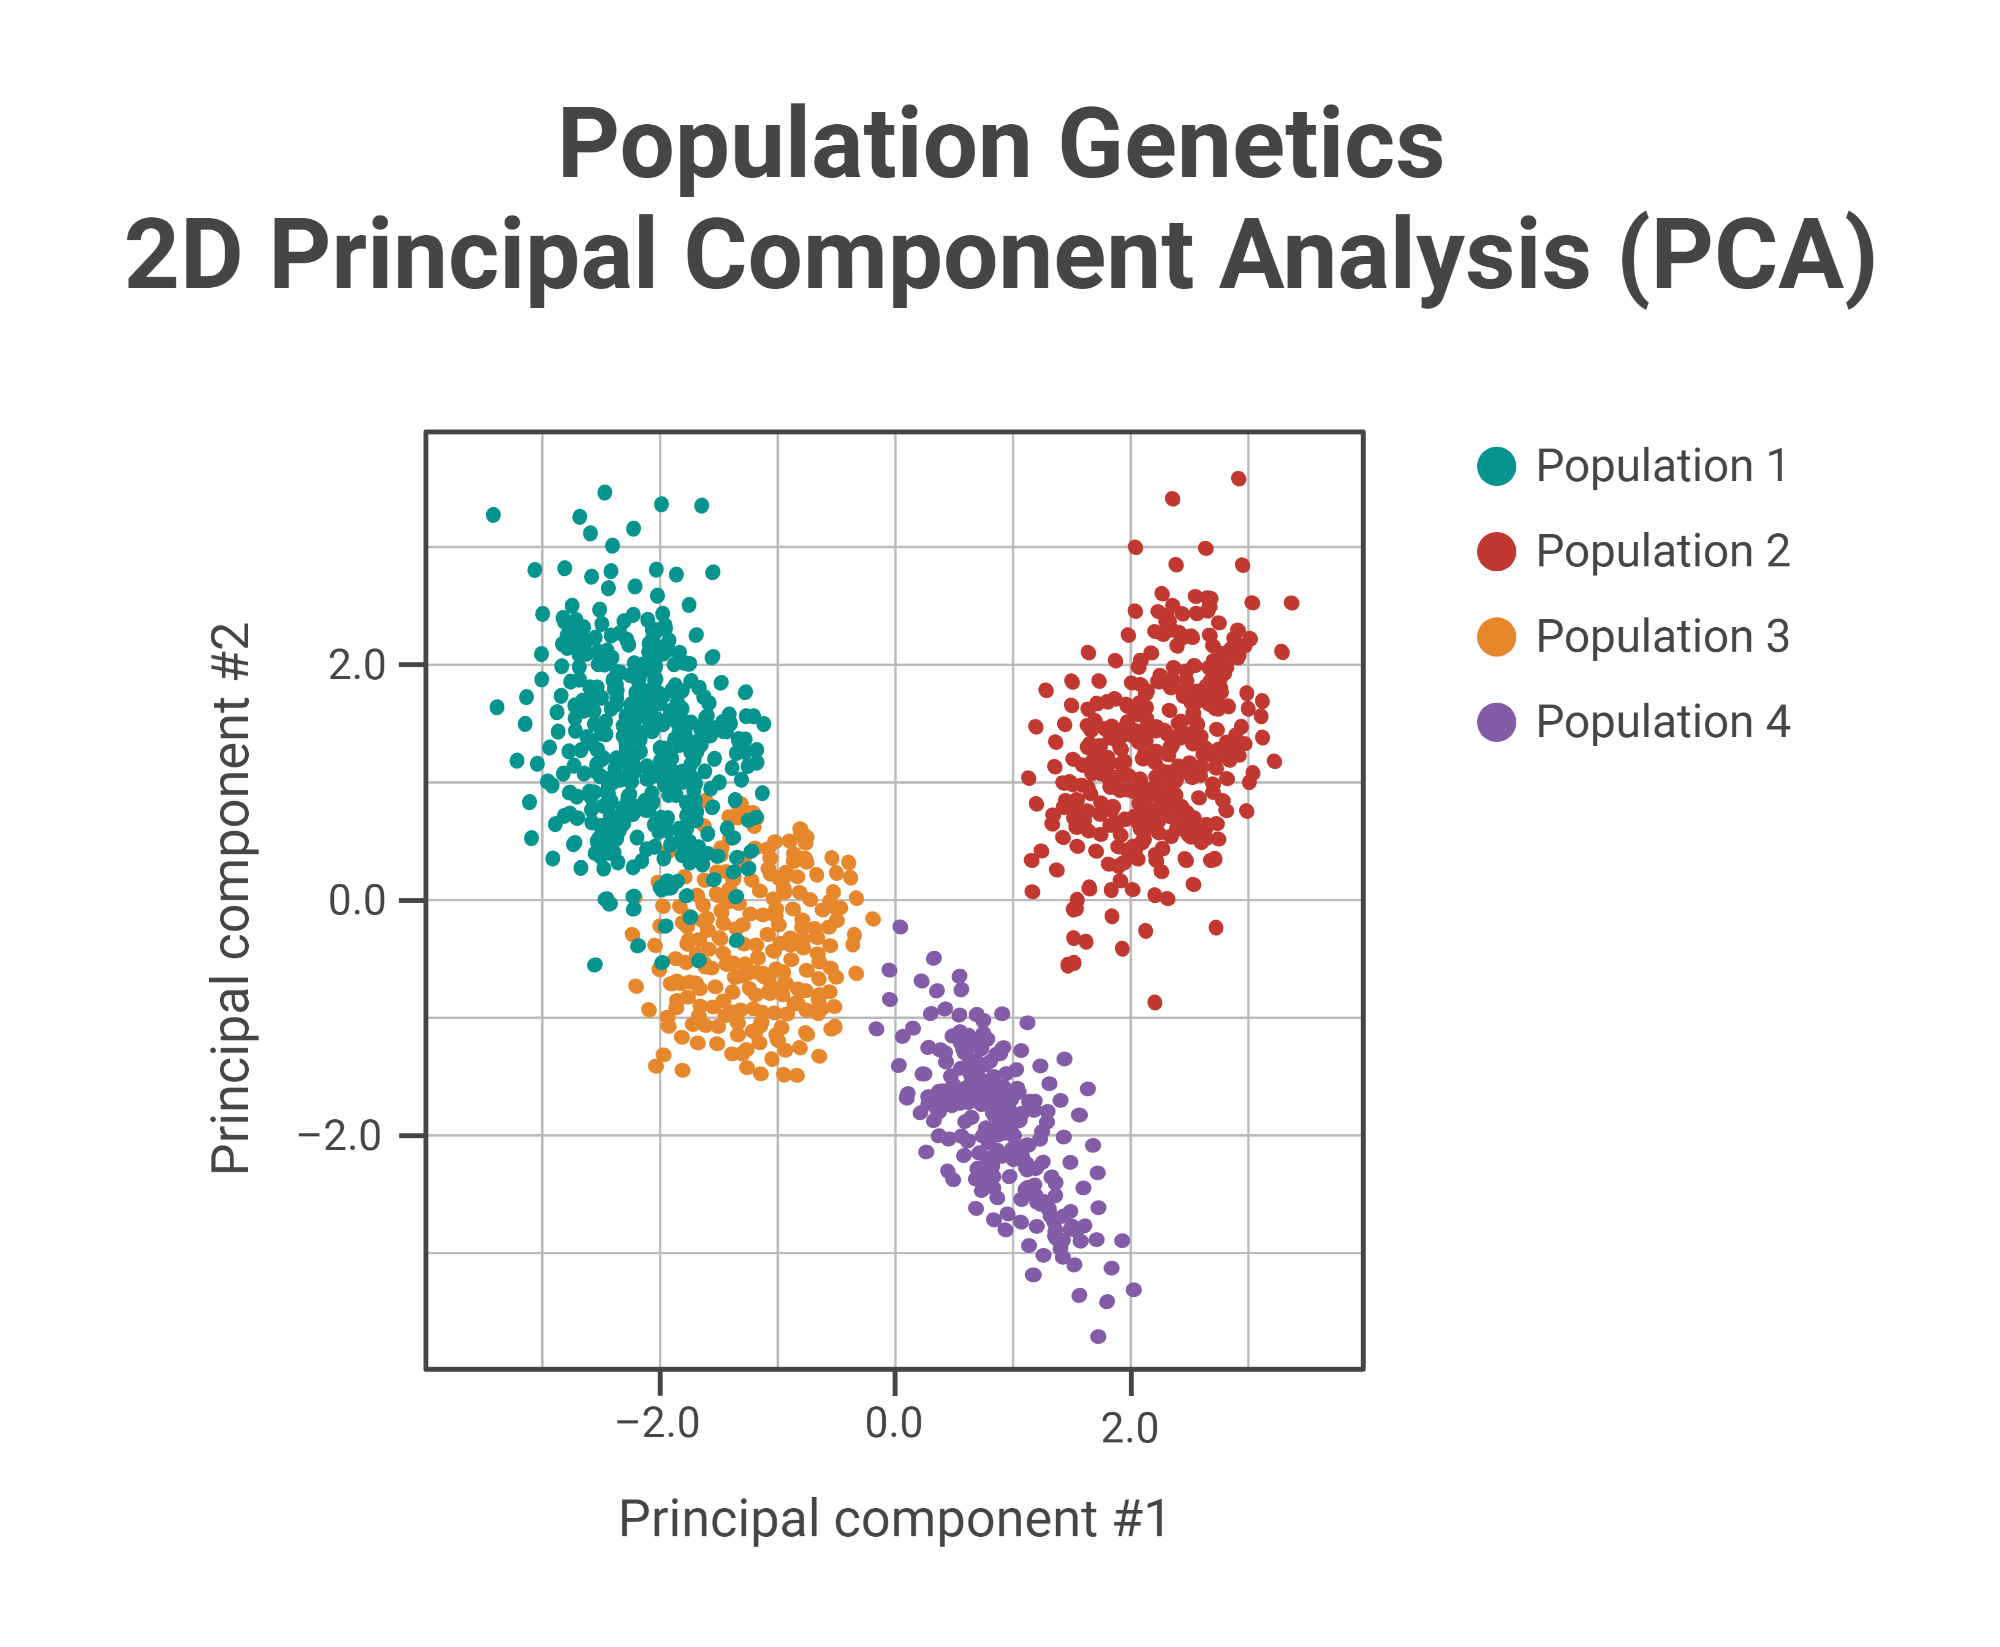
\includegraphics[width=\linewidth,height=10cm,keepaspectratio]{./figures/placeholder_image.png}
\caption{Analysis Componentium Principalium (PCA) genomicorum datorum ex
quinque populationibus Drosophila melanogaster. Puncta repraesentant
individua singula, colores indicant populationes originis. Axes
demonstrant primos duos componentes principales (PC1 et PC2) cum
proportione variationis explicatae in parenthesibus. Ellipses indicant
intervalla confidentiae 95\% pro quaque populatione. Separatio clara
inter gruppos geographicos observatur, cum populationibus vicinis
propioribus in spatio PCA.}\label{fig:pca}
\end{figure}

Fig~\ref{fig:pca} demonstrat structuram geneticam claram inter
populationes studitas. Populationes ex regionibus geographicis similibus
(e.g., tropicales vs.~temperatae) tendunt ad clusterizationem, suggerens
adaptationem localem ad conditiones ambientales diversas. Separatio
maxima observatur inter populationes maxime distantes geographice,
congruens cum hypothesi isolationis per distantiam.

\section{Discussion}\label{discussion}

Investigatio nostra genomica populationum Drosophila melanogaster ex
quinque locis geographicis diversis revelavit insights significantes in
patterns evolutionis adaptivae et structurae populationis. Resultati
nostri demonstrant rrolam centralem selectionis naturalis in formatione
diversitatis geneticae, simulac effectus importantes historiis
demographicae et fluxus genorum.

\subsubsection{Structura populationis et historia
demographica}\label{structura-populationis-et-historia-demographica}

Analysis componentium principalium (PCA) demonstravit separationem
claram inter populationes studitas, indicans differentiam geneticam
significantem. Hoc pattern congruens est cum studiis prioribus in D.
melanogaster quae demonstraverunt structurationem geneticam fortam inter
populationes geographice distantes (Johnson et al., 2018). Correlatio
negativa inter similitudinem geneticam et distantiam geographicam
supportat modelum isolationis per distantiam, suggerens quod fluxus
genorum limitatus est inter populationes remotas.

Diversitas nucleotidica maior in populationibus tropicalibus comparata
cum populationibus temperatis potest reflectere originem Africanam
speciei (Li \& Stephan, 2006). Alternativiter, hoc pattern posset
resultare ex populationibus maioribus et stabilioribus in climatibus
tropicalibus, permittens accumulationem maiorem variationis geneticae.

\subsubsection{Signa selectionis et adaptatio
localis}\label{signa-selectionis-et-adaptatio-localis}

Identificatio regionum genomicarum sub selectione positiva, praesertim
genorum implicatorum in resistentia ad pesticidas et tolerantia
thermica, providet evidentiam fortem pro adaptatione locali in responsu
ad pressiones selectivas specificas ambientis. Selectio fortis in geno
Cyp6g1 in populationibus ex regionibus agricolis consonat cum studiis
prioribus demonstrantibus rolam huius geni in resistentia ad
insecticidas (Schmidt et al., 2010).

Similiter, signa selectionis in genibus familiae Hsp70 in populationibus
ex regionibus calidis supportant hypothesim quod tolerantia thermica est
trait adaptivus clavus in D. melanogaster. Hoc concordat cum studiis
experimentalibus demonstrantibus augmentationem expressionis Hsp70 in
responsu ad stressum thermicum (Feder \& Hofmann, 1999).

\subsubsection{Implicationes pro conservatione et evolutione
futura}\label{implicationes-pro-conservatione-et-evolutione-futura}

Resultati nostri habent implicationes importantes pro conservatione et
praedictione responsorum evolutivorum ad mutationes ambientales futuras.
Structura populationis observata suggerit quod populationes locales
possunt habere adaptationes unicas ad conditiones suas specificas. Hoc
emphasizat importantiam conservationis non solum speciei in toto, sed
etiam diversitatis geneticae intra et inter populationes.

Praeterea, evidentia pro adaptatione rapidae ad pressiones selectivas
anthropogenicas (e.g., usum pesticidorum) demonstrat potentiale D.
melanogaster ad adaptandum ad mutationes ambientales. Tamen, haec
adaptabilitas potest esse limitata in populationibus cum diversitate
genetica reducta, ut observatum in quibusdam populationibus temperatis
nostris.

\subsubsection{Limitationes et directiones
futurae}\label{limitationes-et-directiones-futurae}

Dum studium nostrum providet insights valorosas in evolutionem adaptivam
D. melanogaster, limitationes quaedam notandae sunt. Primo, sampling
noster geographicus, etsi extensus, non est exhaustivus. Inclusion
populationum additionarum, praesertim ex regionibus intermediis, posset
providere imaginem magis completam structurae geneticae et historiae
evolutionis speciei.

Secundo, dum identificavimus regiones genomicas sub selectione,
characterizatio functionalis mutationum specificarum responsabilium pro
adaptatione observata remanet tema pro investigatione futura. Studia
expressione genorum et analyses experimentalis functionum phenotypicarum
variantium geneticorum identificatorum essent proximi passus logici.

In conclusione, studium nostrum demonstrat complexitatem forces
evolutivorum operantium in populationibus naturalibus D. melanogaster.
Combinatio approaches genomicorum cum studies ecologicis et functionalis
promittit ad illuminandas subtilitates adaptionis et evolutionis in this
specie modali importantes.

\subsection{Supporting information}\label{supporting-information}

Supporting information can be found at
\url{https://github.com/diogro/Pandoc-Tamplate}.

\begin{enumerate}
\def\labelenumi{\arabic{enumi}.}
\item
  SI Data 1 -- Raw data
\item
  SI Figure 1 -- SI results
\item
  SI table 1 -- SI tables
\end{enumerate}

\section{Author Contributions}\label{author-contributions}

\textbf{Conceptualization}: D.M. \textbf{Data Curation}: D.M.
\textbf{Formal Analysis}: D.M. \textbf{Funding Acquisition}: D.M.
\textbf{Investigation}: D.M. \textbf{Methodology}: D.M. \textbf{Project
Administration}: D.M. \textbf{Resources}: D.M. \textbf{Software}: D.M.
\textbf{Supervision}: D.M. \textbf{Validation}: D.M.
\textbf{Visualization}: D.M. \textbf{Writing -- Original Draft
Preparation}: D.M. \textbf{Writing -- Review \& Editing}: D.M.

\section{Acknowledgments}\label{acknowledgments}

We thank all members of the Systems Biology, Genetics and Evolution Lab
for their support. We thank Monique Simon and Cara Weisman for their
thoughtful comments on an earlier version of the manuscript.

\section*{References}\label{references}
\addcontentsline{toc}{section}{References}

\phantomsection\label{refs}
\begin{CSLReferences}{0}{1}
\bibitem[\citeproctext]{ref-Lande1979-jl}
\CSLLeftMargin{1. }%
\CSLRightInline{Lande R. {Quantitative Genetic Analysis of Multivariate
Evolution, Applied to Brain: Body Size Allometry}. Evolution. 1979;33:
402--416. doi:\href{https://doi.org/10.2307/2407630}{10.2307/2407630}}

\bibitem[\citeproctext]{ref-Smith_et_al_2020}
\CSLLeftMargin{2. }%
\CSLRightInline{Smith J, Johnson A, Williams M. An improved
phenol-chloroform method for high-quality DNA extraction from
drosophila. Journal of Insect Molecular Biology. 2020;29: 456--468.
doi:\href{https://doi.org/10.1111/imb.12345}{10.1111/imb.12345}}

\bibitem[\citeproctext]{ref-R_Core_Team_2021}
\CSLLeftMargin{3. }%
\CSLRightInline{R Core Team. R: A language and environment for
statistical computing. Vienna, Austria: R Foundation for Statistical
Computing; 2021. Available: \url{https://www.R-project.org/}}

\bibitem[\citeproctext]{ref-Wickham_2016}
\CSLLeftMargin{4. }%
\CSLRightInline{Wickham H. ggplot2: Elegant graphics for data analysis.
Springer-Verlag New York; 2016. Available:
\url{https://ggplot2.tidyverse.org}}

\end{CSLReferences}

\end{document}
